\chapter{Scattering}
\section{Free Electron}
Suppose there is an electron traveling with a momentum $k$ without experiencing the potential energy ($U=0$). At $t=0$, the scattering happens and the momentum changes from $k$ to $k'$ as shown in Fig. 3.1.
\begin{figure}[tbp]
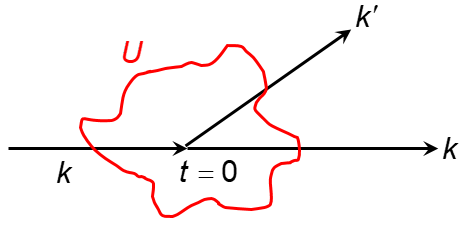
\includegraphics[width=0.4\textwidth]{figures/Fig3_1}
\centering
\caption{\small The electron with a momentum $k$ and the scattering happens at $t = 0$.}
\end{figure}
Thus, \begin{align}
    \big|\psi(x,t)\big>& = \sum_{k}{c_{k}(t)}\big|\phi_{k}(x)\big>\nonumber\\
    & = c_{k}(t)\big|\phi_{k}(x)\big>\text{,}\quad\text{$t=0$}\nonumber\\
    & = \big|\phi_{k}(x)\big> = e^{ikx}
\end{align} where \begin{equation}
    c_{k}(0)=
    \begin{cases}
    1 & \text{for momentum$=k$ since we already knew $k$}\\
    0 & \text{for every other momentum}
    \end{cases}
\end{equation} The Schrodinger equation tells \begin{equation}
    i\hbar\frac{\partial}{\partial t}\big|\psi(x,t)\big> = -\frac{\hbar^{2}}{2m_{0}}\nabla^{2}\big|\psi(x,t)\big>\nonumber
\end{equation} \begin{equation}
    \Rightarrow\sum_{k}{i\hbar\frac{\partial}{\partial t}c_{k}\big|\phi_{k}(x,t)\big>} = \sum_{k}{-\frac{\hbar^{2}}{2m_{0}}\nabla^{2}c_{k}\big|\phi_{k}(x,t)\big>}\nonumber
\end{equation} \begin{equation}
    \Rightarrow\sum_{k}{\big|\phi_{k}(x,t)\big>i\hbar\frac{\partial}{\partial t}c_{k}} = \sum_{k}{c_{k}\varepsilon_{k}\big|\phi_{k}(x,t)\big>}
\end{equation} $\big<\phi_{k}'(x,t)\big|$: \begin{equation}
    i\hbar\frac{\partial}{\partial t}c_{k'} = c_{k'}\varepsilon_{k'}\nonumber
\end{equation} \begin{equation}
    \Rightarrow\frac{\partial}{\partial t}c_{k'} = -i\omega_{k'}c_{k'}\nonumber
\end{equation} \begin{equation}
    \Rightarrow\boxed{c_{k'}(t) = c_{k'}(0)e^{-i\omega_{k'}t}}
\end{equation}
\section{Electron Experiencing Potential}
If $U\neq 0$ and is a function of both position $x$ and time $t$, the Schrodinger's equation becomes \begin{equation}
    i\hbar\frac{\partial}{\partial t}c_{k}(t)\big|\phi_{k}(x)\big> = -\frac{\hbar^{2}}{2m_{0}}\nabla^{2}c_{k}(t)\big|\phi_{k}(x)\big> + Uc_{k}(t)\big|\phi_{k}(x)\big>
\end{equation} $\big<\phi_{k}'(x,t)\big|$: \begin{equation}
    i\hbar\frac{\partial}{\partial t}c_{k'} = c_{k'}\varepsilon_{k'} + \sum_{k}{\big<\phi_{k'}\big|U\big|\phi_{k}\big>c_{k}}
\end{equation} If $\big<\phi_{k'}\big|U\big|\phi_{k}\big>\equiv U_{k'k}(t)$ and $\frac{\varepsilon_{k'}}{\hbar}\equiv \omega_{k'}$, then \begin{equation}
    \boxed{\frac{\partial}{\partial t}c_{k'} + i\omega_{k'}c_{k'} = \frac{1}{i\hbar}\sum_{k}{U_{k'k}c_{k}}}
\end{equation} The general solution of the Equation (3.7) is \begin{equation}
    c_{k'}(T) = e^{-i\omega_{k'}T}\int_{0}^{T}dt\sum_{k}{\frac{U_{k'k}}{i\hbar}c_{k}e^{i\omega_{k'}t}}
\end{equation} Since the solution $c_{k'}$ contains itself $c_{k}$, the iteration is needed to get $c_{k'}$. Here, we adopt the $c_{k}$ for the free electron Hamiltonian [Equation (3.4)] as a first-order approximation. Thus, \begin{equation}
    \boxed{c_{k'}(T) = e^{-i\omega_{k'}T}\int_{0}^{T}dt\sum_{k}{\frac{U_{k'k}}{i\hbar}e^{i(\omega_{k'}-\omega_{k})t}}}
\end{equation} The scattering probability $P_{k'k}^{T}$ is \begin{equation}
    P_{k'k}^{T} = c_{k'}c_{k} = \frac{1}{\hbar^{2}}\big|\int_{0}^{T}\sum_{k}{U_{k'k}e^{i(\omega_{k'}-\omega_{k})t}}dt\big|^{2}
\end{equation} and the scattering rate $S_{k'k}$ is\footnote{The same results can be obtained using the {\bf Perturbation Theory}. In fact, the first order approximation used in the Equation (3.9) is the perturbation theory itself.} \begin{equation}
    \boxed{S_{k'k} = \frac{P_{k'k}^{T}}{T} = \frac{1}{T\hbar^{2}}\big|\int_{0}^{T}\sum_{k}{U_{k'k}e^{i(\omega_{k'}-\omega_{k})t}}dt\big|^{2}}
\end{equation}
\subsubsection{If $U_{k'k}$ is only a function of $x$}
In practical cases, this approximation is valid since the impurities cannot move in the solids. The $U_{k'k}$ can be taken out from the integration in the Equation (3.11). Thus, \begin{equation}
    S_{k'k} = \frac{1}{T\hbar^{2}}\sum_{k}\big|U_{k'k}\big|^{2}\big|\int_{0}^{T}e^{i\omega t}dt\big|^{2}
\end{equation} where $\omega \equiv \omega_{k'}-\omega_{k}$. The integration in the Equation (3.12) can be evaluated analytically\footnote{This is not a delta function since $T$ is not infinity.} \begin{align}
    \big|\int_{0}^{T}e^{i\omega t}dt\big|^{2}& = \big|\int_{0}^{T}(\cos{\omega t}+i\sin{\omega t})dt\big|^{2}\nonumber\\
    & = \frac{2}{\omega^{2}}(1-\cos{\omega T}) = \frac{\sin{\frac{\varepsilon T}{2\hbar}}^{2}}{(\frac{\varepsilon T}{2\hbar})^{2}}T^{2}
\end{align} where $\varepsilon \equiv \hbar \omega$. The function of $\frac{\sin{x}^{2}}{x^{2}}$ is shown in Fig. 3.2.
\begin{figure}[tbp]
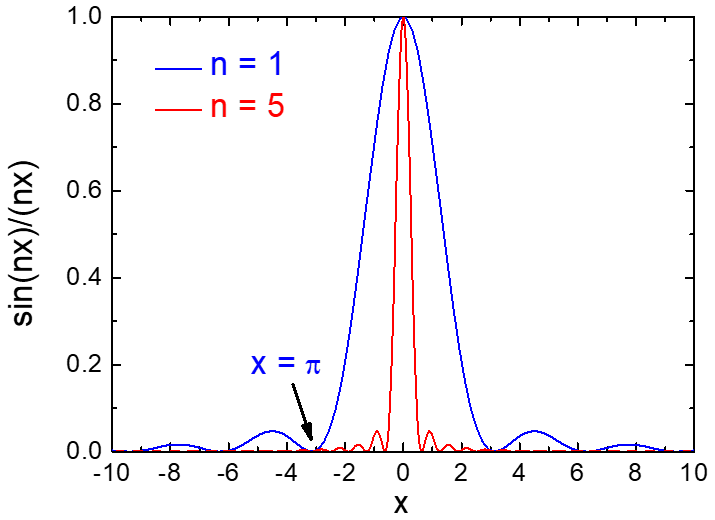
\includegraphics[width=0.6\textwidth]{figures/Fig3_2}
\centering
\caption{\small $\frac{\sin{nx}}{nx}$ versus $x$ at $n = 1$ and $5$. When $n$ is large, the function approaches to the delta function. In other words, if $\frac{\varepsilon T}{2\hbar}\gg\pi$, $\frac{\sin{x}}{x}$ becomes the delta function.}
\end{figure}
When $T \gg \frac{2\pi\hbar}{\varepsilon} ~ \text{f-sec}$, $\frac{\sin{\frac{\varepsilon T}{2\hbar}}^{2}}{(\frac{\varepsilon T}{2\hbar})^{2}}$ can be approximated as a delta function. This approximation is valid in electronics since the scattering time is in order of p-sec. However, in optoelectronics, this approximation is not good because the scattering time as faster as f-sec is possible. To ensure that the integration is not changed after replacing $\frac{\sin{\frac{\varepsilon T}{2\hbar}}^{2}}{(\frac{\varepsilon T}{2\hbar})^{2}}$ with a delta function, the area under the function should be obtained \begin{equation}
    \int \frac{\sin{\frac{\varepsilon T}{2\hbar}}^{2}}{(\frac{\varepsilon T}{2\hbar})^{2}}d\varepsilon = \int \frac{\sin{x}^{2}}{x^{2}}dx \frac{2\hbar}{T}
\end{equation} The above equation can be evaluated using the following trick \begin{equation}
    I(a)\equiv \int\frac{\sin{ax}^{2}}{x^{2}}dx
\end{equation} \begin{equation}
    \frac{dI}{da} = 2\int \frac{\sin{ax}}{x}dx = \pi \Rightarrow I(a) = a\pi
\end{equation} Then, \begin{equation}
    \int \frac{\sin{x}^{2}}{x^{2}}dx \frac{2\hbar}{T} = \frac{2\pi\hbar}{T}
\end{equation} Thus, \begin{equation}
    S_{k'k} = \frac{1}{T\hbar^{2}}\frac{2\pi\hbar}{T}\sum_{k}{\big|U_{k'k}\big|^{2}\delta(\varepsilon_{k'}-\varepsilon_{k})}T^{2}\nonumber
\end{equation}
Or \begin{equation}
    \boxed{S_{k'k} = \frac{2\pi}{\hbar}\sum_{k}{\big|U_{k'k}\big|^{2}\delta(\varepsilon_{k'}-\varepsilon_{k})}}
\end{equation} which is called the {\bf Fermi Golden Rule}. From the above equation, if the potential is time-independent, the scattering will be elastic without losing or gaining any energy.
\subsubsection{If $U_{k'k}$ is only a function of $t$}
If the solid is illuminated by the light or is emitting the photons, the potential will be time-dependent. The potential $U_{k'k}$ can be generally expanded by the Fourier series \begin{equation}
    U_{k'k} = g(t) = \sum_{\omega}{g_{\omega}e^{i\omega t}} + \sum_{\omega}{g_{-\omega}e^{-i\omega t}}
\end{equation} Then, \begin{align}
    S_{k'k}& = \frac{1}{T\hbar^{2}}\sum_{k,\omega}{\big|g_{\omega}^{k'k}\big|^{2}\big|\int_{0}^{T}e^{i(\omega_{k'}-\omega_{k}+\omega)t}dt\big|^{2}+\big|g_{-\omega}^{k'k}\big|^{2}\big|\int_{0}^{T}e^{i(\omega_{k'}-\omega_{k}-\omega)t}dt\big|^{2}}\nonumber\\
    & = \frac{2\pi}{\hbar}\sum_{k,\omega}{\big|g_{\omega}^{k'k}\big|^{2}\delta(\varepsilon_{k'}-\varepsilon_{k}+\hbar\omega)}+\frac{2\pi}{\hbar}\sum_{k,\omega}{\big|g_{-\omega}^{k'k}\big|^{2}\delta(\varepsilon_{k'}-\varepsilon_{k}-\hbar\omega)}
\end{align} The first term in the Equation (3.20) represents the emission process since \begin{equation}
    \varepsilon_{k'} = \varepsilon_{k} - \hbar\omega \nonumber
\end{equation} and the second term represents the absorption process since \begin{equation}
    \varepsilon_{k'} = \varepsilon_{k} + \hbar\omega \nonumber
\end{equation} Note that the cross term in the Equation (3.20) is ignored since physically the absorption and emission processes cannot happen simultaneously.
\section{Master Equation}
Since the scattering changes the momentum from $k$ to $k'$, the distribution function of the electron also changes obeying the {\bf Mater Equation} \begin{equation}
    \frac{df_{k}}{dt} = \sum_{k'}{S_{kk'}f_{k'}(1-f_{k})} - \sum_{k'}{S_{k'k}f_{k}(1-f_{k'})}
\end{equation} where the first and second terms on the right side represent the scattering from $k'$ to $k$ and from $k$ to $k'$. At equilibrium, $\frac{df_{k}}{dt}=0$. Thus, \begin{equation}
    S_{kk'}f_{k'}(1-f_{k}) = S_{k'k}f_{k}(1-f_{k'})\nonumber
\end{equation} or, \begin{align}
    \frac{S_{kk'}}{S_{k'k}}& = \frac{\frac{f_{k}}{1-f_{k}}}{\frac{f_{k'}}{1-f_{k'}}} = \frac{e^{-(\varepsilon_{k}-\mu)/k_{B}T}}{e^{-(\varepsilon_{k'}-\mu)/k_{B}T}} = e^{(\varepsilon_{k'}-\varepsilon_{k})/k_{B}T} = e^{\hbar\omega/k_{B}T}
\end{align} where $f_{k} = 1/[1+e^{(\varepsilon_{k}-\mu)/k_{B}T}]$ and $\varepsilon_{k'}-\varepsilon_{k}\equiv \hbar\omega$. The Equation (3.22) indicates the restoration of the equilibrium. In other words, the probability of going from the higher energy state to the lower is proportional to $e^{\hbar\omega/k_{B}T}$. Recall the Equation (3.20). The emission and absorption have a similar relation \begin{equation}
    \frac{\big|g_{\omega}\big|^{2}}{\big|g_{-\omega}\big|^{2}} = e^{\hbar\omega/k_{B}T}
\end{equation} Since $f_{k}$ is not a function of $k'$, it can be taken out from the summation. Thus, the Master equation becomes \begin{equation}
    \boxed{\frac{df_{k}}{dt} + \frac{f_{k}}{\tau} = \sum_{k'}{S_{kk'}f_{k'}(1-f_{k})}}
\end{equation} where \begin{equation}
    \frac{1}{\tau} = \sum_{k'}{S_{k'k}(1-f_{k'})}
\end{equation} is the lifetime ($\tau$) of the electron due to the scattering. The general solution of the Equation (3.24) is \begin{equation}
    f_{k} = e^{-T/\tau}\int_{0}^{T}e^{t/\tau}\sum_{k'}{S_{kk'}f_{k'}(1-f_{k})}dt
\end{equation} Again, the Equation (3.26) needs to be solved numerically. Let's consider a simplified case: if an electron is coming with the momentum $k$, we have \begin{equation}
    \begin{cases}
    f_{k} = 1 & \text{for momentum$=k$ since we already knew $k$}\\
    f_{k'} = 0 & \text{for every other momentum $k'$}
    \end{cases}
\end{equation} Thus, \begin{equation}
    1-f_{k}\approx 0 \Rightarrow \frac{df_{k}}{dt} + \frac{f_{k}}{\tau} = 0 \Rightarrow f_{k}(t) = f_{k}(0)e^{-t/\tau}
\end{equation}
\section{Relaxation Time}
The relaxation time is the time that a physical quantity $\vec{A}$ is back to the thermal equilibrium and follows \begin{equation}
    \frac{d\big<\vec{A}\big>}{dt} = \frac{\big<\vec{A}\big>-\big<\vec{A_{0}}\big>}{\tau_{A}}
\end{equation} where $\tau_{A}$ is the relaxation time and \begin{equation}
    \big<\vec{A}\big> = \big<\psi\big|A\big|\psi\big> = \text{Trace}(A\rho)
\end{equation} Assume that there is no off-diagonal elements \begin{equation}
    \big<A\big>_{k} = \big<\psi_{k}\big|A\big|\psi_{k}\big> = f_{k}A_{k}
\end{equation} Thus, \begin{equation}
    \frac{d\big<\vec{A}\big>}{dt} = \frac{d}{dt}\sum_{k}{\big<A\big>_{k}} = \frac{d}{dt}\sum_{k}{f_{k}A_{k}}
\end{equation} Multiplying $\sum_{k}{A_{k}}$ to the Master equation, we have \begin{align}
    \sum_{k}{\frac{d}{dt}f_{k}A_{k}}& = \sum_{kk'}{\underbrace{S_{kk'}f_{k'}(1-f_{k})A_{k}}_{=S_{k'k}f_{k}(1-f_{k'})A_{k'}}} - \sum_{kk'}{S_{k'k}f_{k}(1-f_{k'})A_{k}}\nonumber\\
    & = \sum_{kk'}{S_{k'k}f_{k}(1-f_{k'})[A_{k'}-A_{k}]} = \frac{\big<\vec{A}\big>-\big<\vec{A_{0}}\big>}{\tau_{A}}
\end{align} Hence, \begin{align}
    \frac{1}{\tau_{A}}& = \frac{\sum_{kk'}{S_{k'k}f_{k}(1-f_{k'})[A_{k'}-A_{k}]}}{\big<\vec{A}\big>-\big<\vec{A_{0}}\big>}\nonumber\\
    & = \frac{\sum_{kk'}{S_{k'k}f_{k}(1-f_{k'})[A_{k'}-A_{k}]}}{\sum_{k}{f_{k}A_{k}}-\sum_{k}{f_{k0}A_{k}}}\nonumber\\
    & = \frac{\sum_{kk'}{S_{k'k}f_{k}(1-f_{k'})}}{\sum_{k}{f_{k}-f_{k0}}}\left[1-\frac{A_{k'}}{A_{k}}\right]\nonumber\\
    & = \sum_{k}{\frac{1}{\tau_{A}}(k)}
\end{align} where $\frac{1}{\tau_{k}}(k)$ is the $k$-dependent relaxation time \begin{equation}
    \boxed{\frac{1}{\tau_{A}}(k) = \sum_{k'}{\frac{S_{k'k}f_{k}(1-f_{k'})}{f_{k}-f_{k0}}\left[1-\frac{A_{k'}}{A_{k}}\right]}}
\end{equation}
\section{Phonons}
The phonons are the quantized quasi-particles that represent the lattice vibration. The one-dimensional lattice can be modeled as the atoms connected to each other by the springs as shown in Fig. 3.3.
\begin{figure}[tbp]
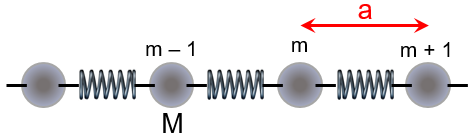
\includegraphics[width=0.6\textwidth]{figures/Fig3_3}
\centering
\caption{\small One dimensional lattice (lattice constant is $a$) with the springs connecting each atom with the mass $M$.}
\end{figure}
The force equation says \begin{equation}
    F = M\frac{d^{2}x_{m}}{dt^{2}} = K\left[(x_{m+1}-x_{m})-(x_{m}-x_{m-1})\right]
\end{equation} where $K$ is the spring constant and the $x$ is the position of the atom. The solution of the Equation (3.36) is \begin{align}
    \widetilde{x_{m}}& = \widetilde{x}e^{i(\beta ma - \omega t)} + \widetilde{x}^{*}e^{-i(\beta ma - \omega t)}\nonumber\\
    & = 2\big|\widetilde{x}\big|\cos{(\beta ma - \omega t + \phi)} \equiv 2\big|\widetilde{x}\big|\cos{\theta}
\end{align} where $\widetilde{x}$ is the amplitude, $\beta$ is the momentum, and $phi$ is the phase. To determine the dispersion relation of phonons, we take the derivative to the Equation (3.37) with respect to time $t$ twice and equate it to the Equation (3.36) \begin{equation}
    2\big|\widetilde{x_{m}}\big|(-\cos{\theta})(-\omega)(-\omega) = -\frac{K}{M}2\big|\widetilde{x_{m}}\big|4\cos{\theta}\sin^{2}{\frac{\beta a}{2}}
\end{equation} Thus, the dispersion relation is \begin{equation}
    \boxed{\omega(\beta) = 2\sqrt{\frac{K}{M}}\sin{\frac{\beta a}{2}}}
\end{equation} When $\omega$ is close to zero, the Equation (3.39) can be expanded as a straight line. In other words, \begin{equation}
    \omega \propto \beta \quad \Rightarrow \quad \omega = c_{S}\beta
\end{equation} where $c_{S}$ is the velocity of sound since the Equation (3.39) represents the acoustic phonon mode where all the atoms move in the same direction. For optical phonon mode, the frequency $\omega$ is nearly a constant say $\omega_{0}$ and the two atoms move in the opposite direction. The kinetic energy of an atom in the acoustic mode at momentun $\beta$ is \begin{equation}
    \frac{1}{2}Mv^{2} = 2M\big|\widetilde{x_{\beta}}\big|^{2}\omega_{\beta}^{2}\sin^{2}{(\overset{\rightharpoonup}{\beta}\cdot\overset{\rightharpoonup}{r}-\omega_{\beta}t)}
\end{equation} If there are $N$ atoms, the total energy will be \begin{align}
    E^{\text{total}}& = 2M\big|\widetilde{x_{\beta}}\big|^{2}\omega_{\beta}^{2}N,\quad MN\equiv \rho V \nonumber\\
    & = 2\rho V \big|\widetilde{x_{\beta}}\big|^{2}\omega_{\beta}^{2}\nonumber\\
    & = n_{\beta}\hbar\omega_{\beta}
\end{align} where $\rho$ is the mass density and $n_{\beta}$ is the number of phonons (fermion) \begin{equation}
    n_{\beta} = \frac{1}{e^{\frac{\hbar\omega_{\beta}}{k_{B}T}}-1}
\end{equation} Hence, \begin{equation}
    \big|\widetilde{x_{\beta}}\big|^{2} = \frac{\hbar n_{\beta}}{2\rho V \omega_{\beta}}
\end{equation} and \begin{equation}
    \widetilde{x_{\beta}}(\overset{\rightharpoonup}{r},t) = \sqrt{\frac{\hbar}{2\rho V\omega_{\beta}}}\left[a_{\beta}e^{i(\overset{\rightharpoonup}{\beta}\cdot\overset{\rightharpoonup}{r}-\omega_{\beta}t)}+a_{\beta}^{*}e^{-i(\overset{\rightharpoonup}{\beta}\cdot\overset{\rightharpoonup}{r}-\omega_{\beta}t)}\right]
\end{equation} where \begin{equation}
    a_{\beta}^{*}a_{\beta} = n_{\beta} = \frac{1}{e^{\frac{\hbar\omega_{\beta}}{k_{B}T}}-1}
\end{equation}
\subsection{Electron-Phonon Scattering}
The electron-phonon scattering potential $U_{\beta}^{S}$ can be approximated as \begin{align}
    U_{\beta}^{S}(\overset{\rightharpoonup}{r},t) = K_{\beta}\widetilde{x_{\beta}}(\overset{\rightharpoonup}{r},t)
\end{align} where $K_{\beta}$ is the coupling constant related to the deformation of the lattice. For the acoustic mode, the movement of the atoms imposes the strain on the lattice, and thus \begin{equation}
    U_{\beta}^{S} = D_{a}S_{\beta} = D_{a}(\nabla\cdot\widetilde{x_{\beta}}) = i\beta D_{a}\widetilde{x_{\beta}} \equiv K_{\beta}\widetilde{x_{\beta}}
\end{equation} where $D_{a}$ is the deformation potential and $S_{\beta}$ is the strain. The Equation (3.47) is the result of the Taylor expansion of change in the potential. For the optical phonon mode, the frequency is nearly fixed. Thus, \begin{equation}
    K_{\beta} = D_{o}
\end{equation} Since we assume the phonon modes ($\phi_{k}$) are the plane waves\footnote{S. Datta, Quantum Transport Atom to Transistor, 2005, p. 261.}, we have \begin{align}
    U_{k'k}(t)& = \big<\phi_{k'}\big|U_{\beta}^{S}(\overset{\rightharpoonup}{r},t)\big|\phi_{k}\big>\nonumber\\
    & = K_{\beta}\sqrt{\frac{\hbar}{2\rho V\omega_{\beta}}}\left(\underbrace{\int a_{\beta}^{*}e^{-\overset{\rightharpoonup}{k'}\cdot\overset{\rightharpoonup}{r}}e^{\overset{\rightharpoonup}{-\beta}\cdot\overset{\rightharpoonup}{r}}e^{\overset{\rightharpoonup}{k}\cdot\overset{\rightharpoonup}{r}}e^{i\omega_{\beta}t}}_{\text{emission}}+\underbrace{\int a_{\beta}e^{-\overset{\rightharpoonup}{k'}\cdot\overset{\rightharpoonup}{r}}e^{\overset{\rightharpoonup}{\beta}\cdot\overset{\rightharpoonup}{r}}e^{\overset{\rightharpoonup}{k}\cdot\overset{\rightharpoonup}{r}}e^{-i\omega_{\beta}t}}_{\text{absorption}}\right)
\end{align} and \begin{equation}
    \big|U_{k'k}\big|^{2} = \underbrace{\big|K_{\beta}\big|^{2}\frac{\hbar a_{\beta}a_{\beta}^{*}}{2\rho V\omega_{\beta}}\delta(\overset{\rightharpoonup}{k}-\overset{\rightharpoonup}{k'}-\overset{\rightharpoonup}{\beta})}_{\text{emission}}+\underbrace{\big|K_{\beta}\big|^{2}\frac{\hbar a_{\beta}^{*}a_{\beta}}{2\rho V\omega_{\beta}}\delta(\overset{\rightharpoonup}{k}-\overset{\rightharpoonup}{k'}+\overset{\rightharpoonup}{\beta})}_{\text{absorption}}
\end{equation} From the Equation (3.23), we have\footnote{Conceptually, $a_{\beta}a_{\beta}^{*}$ and $a_{\beta}^{*}a_{\beta}$ are the {\bf lowering operator} and {\bf raising operator} of the simple harmonic oscillator which satisfies $[a_{\beta}a_{\beta}^{*},a_{\beta}^{*}a_{\beta}] = 1$ and thus $a_{\beta}^{*}a_{\beta}=n_{\beta}+1$. See D. J. Griffiths, Introduction to Quantum Mechanics, 2005, p. 43-44.} \begin{equation}
    \frac{\text{emission}=a_{\beta}a_{\beta}^{*}}{\text{absorption}=a_{\beta}^{*}a_{\beta}=n_{\beta}} = e^{\hbar\omega/kT}\quad\Rightarrow\quad a_{\beta}^{*}a_{\beta}=n_{\beta}+1
\end{equation} Therefore, the scattering rate [the Equation (3.20)] becomes \begin{align}
    S_{k'k}& = \underbrace{\sum_{k,\beta}{\frac{\pi(n_{\beta}+1)}{\rho V \omega_{\beta}}\big|K_{\beta}\big|^{2}\delta(\overset{\rightharpoonup}{k}-\overset{\rightharpoonup}{k'}-\overset{\rightharpoonup}{\beta})\delta(\varepsilon_{k'}-\varepsilon_{k}+\hbar\omega_{\beta})}}_{\text{emission}}\nonumber\\
    &\quad +\underbrace{\sum_{k,\beta}{\frac{\pi n_{\beta}}{\rho V \omega_{\beta}}\big|K_{\beta}\big|^{2}\delta(\overset{\rightharpoonup}{k}-\overset{\rightharpoonup}{k'}+\overset{\rightharpoonup}{\beta})\delta(\varepsilon_{k'}-\varepsilon_{k}-\hbar\omega_{\beta})}}_{\text{absorption}}
\end{align} Note that at $T=0$K, the absorption $n_{\beta} = 0$ but the emission $n_{\beta}+1\neq 0$, indicating the spontaneous emission.
\subsection{Simplification of Electron-Phonon Scattering Using Effective Mass Approximation}
Since the Equation (3.53) involves the electronic band structure effect, it's difficult to solve in the real device geometry. Thus, the effective mass approximation is applied to simplify the problem. In the Equation (3.53), the momentum is conserved with the phonon momentum, so the momentum of the emission and absorption processes can be drawn as shown in Fig. 3.4.
\begin{figure}[tbp]
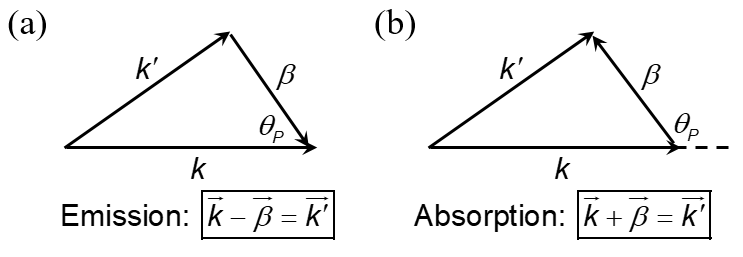
\includegraphics[width=0.6\textwidth]{figures/Fig3_4}
\centering
\caption{\small (a) Phonon emission and (b) absorption processes.}
\end{figure}
From the energy conservation of the emission process, we have \begin{equation}
    \varepsilon_{k'}-\varepsilon_{k}+\hbar\omega_{\beta} = 0\nonumber
\end{equation} \begin{equation}
    \Rightarrow \frac{\hbar^{2}}{2m}\left(k'^{2}-k^{2}+\frac{2m\omega_{\beta}}{\hbar}\right) = 0, \quad k'^{2} = k^{2}+\beta^{2}-2k\beta\cos{\theta_{P}}\nonumber
\end{equation} \begin{equation}
    \Rightarrow \boxed{\cos{\theta_{P}} = \frac{m\omega_{\beta}}{\hbar k \beta}+\frac{\beta}{2k}} \quad \text{For emission}
\end{equation} Similarly, \begin{equation}
    \boxed{\cos{\theta_{P}} = \frac{m\omega_{\beta}}{\hbar k \beta}-\frac{\beta}{2k}} \quad \text{For absorption}
\end{equation}
\subsubsection{Acoustic Phonon}
For acoustic phonon, the dispersion relation can be simplified as [Equation (3.40)]\begin{equation}
    \omega_{\beta} = c_{S}\beta\nonumber
\end{equation} Thus, the momentum $\beta$ for the emission and absorption are \begin{equation}
    \beta^{\text{em}} = 2k\left(\cos{\theta_{P}}-\frac{mc_{S}}{\hbar k}\right)
\end{equation} \begin{equation}
    \beta^{\text{ab}} = 2k\left(\frac{mc_{S}}{\hbar k}-\cos{\theta_{P}}\right)
\end{equation} Since $\cos{\theta_{P}}\leq 1$, for the emission to happen we have \begin{equation}
    \frac{mc_{S}}{\hbar k}<1\quad\Rightarrow\quad\frac{\hbar k}{m}>c_{S}
\end{equation} which is the Cherenkov condition saying that the velocity of the electron should be greater than the sound velocity to emit the acoustic phonon.
\subsubsection{Optical Phonon}
Since the frequency in the optical phonon mode is nearly fixed, we have \begin{equation}
    \cos{\theta_{P}} = \frac{m\omega_{0}}{\hbar k \beta^{\text{em}}}+\frac{\beta^{\text{em}}}{2k}
\end{equation} for the emission. Hence, \begin{equation}
    \beta^{\text{em}} = k\cos{\theta_{P}}\pm\sqrt{k^{2}\cos^{2}{\theta_{P}}-\frac{2m\omega_{0}}{\hbar}}
\end{equation} Since $\cos{\theta_{P}}\leq 1$, for the emission to happen we have \begin{equation}
    \frac{2m\omega_{0}}{\hbar} < k^{2}\quad\Rightarrow\quad\frac{\hbar^{2}k^{2}}{2m}>\hbar\omega_{0}
\end{equation} indicating that the kinetic energy of the electron should be larger than that of the optical phonon for the emission.
\subsubsection{Lifetime of Electron-Phonon Scattering}
If the condition $\overset{\rightharpoonup}{k}-\overset{\rightharpoonup}{k'}\pm\overset{\rightharpoonup}{\beta}=0$ has been held, the Equation (3.53) can be further simplified using the effective mass approximation \begin{align}
    S_{k'k}(k)& = \underbrace{\frac{\pi m}{\rho V\hbar^{2}}\sum_{\beta}{\frac{\big|K_{\beta}\big|^{2}(n_{\beta}+1)}{ \omega_{\beta}k\beta}\delta\left(\cos{\theta_{P}}-\frac{m\omega_{\beta}}{\hbar k\beta}-\frac{\beta}{2k}\right)}}_{\text{emission}}\nonumber\\
    &\quad +\underbrace{\frac{\pi m}{\rho V\hbar^{2}}\sum_{\beta}{\frac{\big|K_{\beta}\big|^{2}n_{\beta}}{ \omega_{\beta}k\beta}\delta\left(\cos{\theta_{P}}-\frac{m\omega_{\beta}}{\hbar k\beta}+\frac{\beta}{2k}\right)}}_{\text{absorption}}
\end{align} Recall the Equations (3.25), (3.27), and (3.28), the lifetime of the electron-phonon scattering is\footnote{Summing over $k'$ is the same as summing over $\beta$.} \begin{equation}
    \frac{1}{\tau(k)} = \sum_{\beta}{S_{k'k}^{\text{em}}}+\sum_{\beta}{S_{k'k}^{\text{ab}}}
\end{equation} and the summation over $\beta$ is \begin{equation}
    \sum_{\beta} \rightarrow \int\frac{d\beta_{x}d\beta_{y}d\beta_{z}}{\frac{2\pi}{L_{x}}\frac{2\pi}{L_{y}}\frac{2\pi}{L_{z}}} = \frac{V}{8\pi^{3}}\int\beta^{2}d\beta(2\pi)\int_{-1}^{1}d\cos{\theta_{P}}
\end{equation} The lifetime of the acoustic phonon emission is \begin{align}
    \frac{1}{\tau^{\text{em}}(k)}& = \frac{\pi m}{\rho V\hbar^{2}}\frac{V}{8\pi^{3}}2\pi\int_{\beta_{\text{min}}}^{\beta_{\text{max}}}\frac{\beta^{2}d\beta\big|K_{\beta}\big|^{2}(n_{\beta}+1)}{\omega_{\beta}k\beta}\int_{-1}^{1}\delta\left(\cos{\theta_{P}}-\frac{m\omega_{\beta}}{\hbar k\beta}-\frac{\beta}{2k}\right)d\cos{\theta_{P}}\nonumber\\
    & = \frac{mD_{a}^{2}}{4\pi\rho\hbar^{2}}\frac{1}{kc_{S}}\int_{\beta_{\text{min}}}^{\beta_{\text{max}}}\beta^{2}d\beta(n_{\beta}+1),\quad \omega_{\beta}=c_{S}\beta\quad\text{and}\quad\big|K_{\beta}\big|^{2}=\beta^{2}D_{a}^{2}
\end{align} For the acoustic phonon, $\hbar\omega_{\beta}\ll k_{B}T$, and thus $n_{\beta}\approx\frac{k_{B}T}{\hbar\omega_{\beta}}\gg 1$ and $n_{\beta}+1\approx n_{\beta}$. Furthermore, $\beta_{\text{max}}^{\text{em}}\approx 2k$ and $\beta_{\text{min}}^{\text{em}}\approx 0$. The Equation (3.65) becomes \begin{align}
    \frac{1}{\tau^{\text{em}}(k)}& = \frac{mD_{a}^{2}}{4\pi\rho\hbar^{3}}\frac{k_{B}T}{kc_{S}^{2}}\int_{0}^{2k}\beta d\beta = \frac{mD_{a}^{2}k_{B}T}{2\pi\rho\hbar^{3}c_{S}^{2}}k
\end{align} Similarly, the lifetime of the absorption is \begin{equation}
    \frac{1}{\tau^{\text{ab}}(k)} = \frac{mD_{a}^{2}k_{B}T}{2\pi\rho\hbar^{3}c_{S}^{2}}k
\end{equation} Therefore, the total lifetime due to the electron-phonon scattering is \begin{align}
    \frac{1}{\tau(k)}& = \frac{mD_{a}^{2}k_{B}T}{\pi\rho\hbar^{3}c_{S}^{2}}k,\quad k=\frac{\sqrt{2mE(k)}}{\hbar}\nonumber\\
    & = \frac{(2mk_{B}T)^{3/2}D_{a}^{2}}{2\pi\rho\hbar^{4}c_{S}^{2}}\sqrt{\frac{E(k)}{k_{B}T}}
\end{align} For GaAs, \begin{equation}
    \tau = 7.6\sqrt{\frac{k_{B}T}{E}}\quad\text{psec}\nonumber
\end{equation}